\documentclass[11pt, a4paper]{beamer}
\usepackage{amsmath}
\usepackage{amsfonts}
\usepackage{amssymb}
\usepackage{tikz}
\usetheme{Frankfurt}
\usecolortheme{seagull}
\usepackage{xltxtra,fontspec}
\usepackage{polyglossia}
\setmainlanguage{english}
\defaultfontfeatures{Scale=MatchLowercase}

\usepackage[absolute,overlay]{textpos}

\setbeamertemplate{footline}
{
  \leavevmode%
  \hbox{%
  \begin{beamercolorbox}[wd=.6\paperwidth,ht=2.25ex,dp=1ex,center]{author in head/foot}%
    \usebeamerfont{author in head/foot}\insertshortauthor
  \end{beamercolorbox}%
  \begin{beamercolorbox}[wd=.4\paperwidth,ht=2.25ex,dp=1ex,center]{title in head/foot}%
    \usebeamerfont{title in head/foot}\insertshorttitle\hspace*{3em}
    \insertframenumber{} / \inserttotalframenumber\hspace*{1ex}
  \end{beamercolorbox}}%
  \vskip0pt%
}


\setbeamertemplate{navigation symbols}{}

\author{Dan Häberlein, Peggy Lucke, J. Nathanael Philipp, Alexander Richter}
\title[The openLegislature project]{Current Topics in Digital Philology\\The openLegislature project}
\date{}
\institute{Universität Leipzig}

%\logo{\includegraphics[scale=0.25]{./LGD_Logo.png}}
%\setbeamersize{text margin left=7mm, text margin right=7mm}

%\usepackage[babel]{csquotes}
%\defbibheading{bibliography}{}
%\bibliography{quellen}

\usepackage[backend=biber,style=numeric]{biblatex}
\addbibresource{lit.bib}

\begin{document}
\section{}
\begin{frame}
\titlepage
\end{frame}

\only<presentation| handout:0> {
	\AtBeginSection[]{%
		\begin{frame}
		\frametitle{Gliederung}
		\tableofcontents[currentsection]
		\end{frame}
	}% AtBeginSection
}

\only<2| handout:1>{
	\begin{frame}
		\frametitle{Outline}
		\tableofcontents
	\end{frame}
}

\section{Introduction}
\subsection{Korpus}
\begin{frame}{Informationen}
\textbf{Plenarprotokolle des Bundestages}
\begin{itemize}
\item stenographische Berichte
\item ab erste Sitzung des Bundestages September 1949
\item vollständig bis zur letzten abgeschlossenen Sitzung
\item PDF-Format
\item aktuelle Wahlperiode auch als Textdatei
\end{itemize}
\end{frame}

\begin{frame}
\textbf{Zugang:}
\begin{itemize}
\item öffentlich
\item frei zugänglich
\item siehe \cite{bundestag} \\[1em]
\end{itemize}
\textbf{Download per Funktionen von:}
\begin{itemize}
\item \textit{Muster:}\\
http://dip21.bundestag.de/dip21/btp/ [Wahlperiode]/[Wahlperiode][Sitzung].pdf
\item \textit{Bsp.:}\\ http://dip21.bundestag.de/dip21/btp/01/01029.pdf\\[1em]
\end{itemize}
\textbf{Größe des Korpus}
\begin{itemize}
\item Momentan 3895 PDF-Dateien
\item Entspricht ca. 10GB
\end{itemize}
\end{frame}

\subsection{Fragestellungen}
\begin{frame}{Welche Fragen können die Informationen des Korpuses beantworten?}

Die ursprüngliche Fragestellung lautete, durch Ähnlichkeitsmessungen von Reden
auf die Herkunft (auf dem Autor, z.B. einem Ghostwriter) der Rede schließen zu
können. Dieses Ziel kann eventuell durch IR Methoden weiterverfolgt werden.  

\textbf{Statistisch:}
\begin{itemize}
\item Wie viele Specher gab es?
\item Wie viele Reden wurden von Mitgliedern einer bestimmten Partei gegeben?
\end{itemize}
\textbf{Schlagwortsuche:}
\begin{itemize}
\item Welcher Redner sprach zu einem bestimmten Sachverhalt?
\item Welche Gesetze wurden zu einem Schlagwort verabschiedet?
\end{itemize}
\end{frame}
\begin{frame}{Warum stellen wir diese Fragen?}
Wir brauchen mehr Transparenz! Wir wollen das was schon da ist, einfacher
zugänglich machen.

Wer hat schon Zeit sich die Reden des Bundestagses anzuhören oder nachzulesen?

\begin{itemize}
\item Interesse zur Politik
\item Analyse des gesprochenen Wortes 
\item Geschichte der deutschen Demokratie greifbar zu machen
\item Transparenz deutscher Politik zu erhöhen
\end{itemize}

Die Politik muss sich langsam dem 21 Jahrhundert annähern. 
2014, also ungefähr nach 20 Jahren Digitales Zeitalter wie wir es heute kennen
werden Wahlen noch immer mit ZETTEL und STIFT geführt!

\end{frame}
\section{Methoden}
\subsection{Vorgehensweise}
\begin{frame}
\frametitle{Methoden 1}
\textbf{Preprocessing:}
\begin{itemize}
\item Lemmatizing
\item ggfs. Part of Speech Analyse  
\item Vergleichen von N-Grammen zur Ähnlichkeitsüberprüfung
\item Keine Stopwortentfernung, da dadurch Informationen verloren gehen!
\end{itemize}
\end{frame}

\begin{frame}
\frametitle{Methoden 2}
\textbf{IR Methoden:}
\begin{itemize}
\item Kookkurrenz auf verschiedenen Ebenen (Reden per Partei, Redner, Gesammt)
\item Clustering
\end{itemize}
\textbf{IR Algorithmen}
\begin{itemize}
\item Ähnlichkeitsmaße berechen und vergleichen 
\item Topic Modell / LDA 
\end{itemize}
\textit {"Latent Dirichlet allocation (LDA) is a generative probabilistic
	model of a corpus. The basic idea is that documents are represented as
 	random mixtures over latent topics, where each topic is characterized by a
 	distribution over words."}, siehe \cite{blatent}
%  	
\end{frame} 

\subsection{Ergebnisse}
\begin{frame}
\frametitle{Vorläufige Ergebnisse}
\begin{itemize}
\item Unstrukturierte Textdateien liegen vor (PDF / TXT)
\item Semistrukturierte XML Dateien aus TXT erzeugt
\item Metadatenbank angelegt
\item Erste einfache XPath Anfragen auf Dateien realisiert 
\end{itemize}
\end{frame}
\begin{frame}
  \frametitle{Architektur Prozess Datenextraktion und -aufbereitung }
  \begin{itemize}
  \item Nutzung des Listener Patterns \cite{javainsel9}
  \item Verwendung der Github-Library Async \cite{async} zur einfachen Erstellung Nebenläufiger Prozessketten
  \end{itemize}  
  \begin{center}
    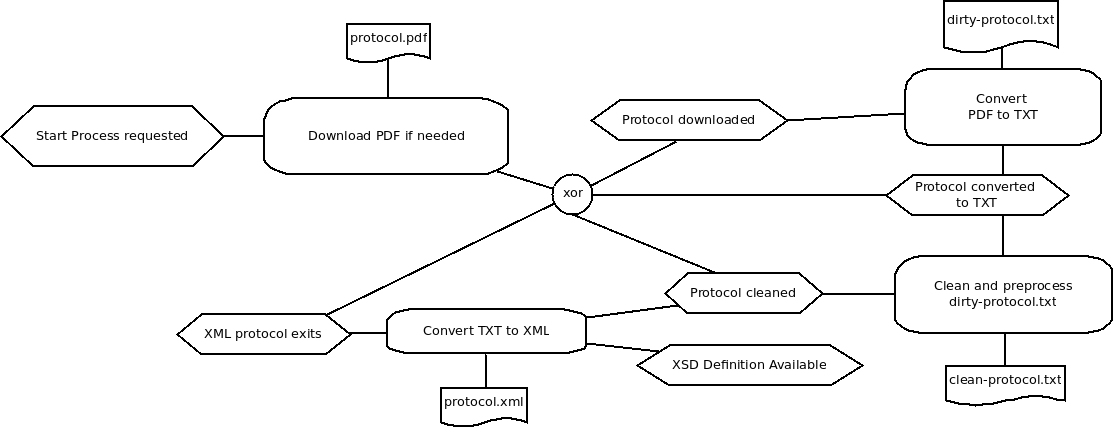
\includegraphics[width=1\textwidth]{../../doc/process-overview.png}
  \end{center}
\end{frame}


\section{Outlook}

\subsection{Anstehende Aufgaben}
\begin{frame}
\frametitle{Ausblick I: nächste Schritte}
Nächste Schritte:
\begin{itemize}
	\item  erweitern der Metadaten-Datenbank mit Metadaten:
		\begin{itemize}
			\item aus bestehenden XML Files
			\item aus zusätzlichen Quellen (z.B. Sitzverteilungen)
	 	\end{itemize}
	\item  Überführen der Strukturierten Daten im XML-Format in einen Document Store
	\item  Analyse der Daten: 
		\begin{itemize}
			\item Clustering (Top-Down, Bottom-Up)
			\item LDA (Latend Dirichlet Allocation)
	 	\end{itemize}
	\end{itemize}
\end{frame}

\subsection{Ziele}
\begin{frame}
\frametitle{Ausblick II: Ziele Vorlesungszeit}

Ziele bis Ende Vorlesungszeit:
\begin{itemize}
	\item XML-Daten in Document-Store ablegen
	\item Metadaten-Datenbank mit weiteren Metadaten erweitern
	\item analysieren der Daten mittels mind. zwei Clustering-Verfahren 
	\item Cluster mit wahrscheinlich gleichen Schreiber (aber nicht Redner) finden und darstellen
\end{itemize}
\end{frame}

\begin{frame}
\frametitle{Ausblick III: Ziele Semester}

Ziele bis Ende Semester:
\begin{itemize}
	\item Analyse mittels LDA
	\item Visualisierung der Ergebnisse der LDA-Analysen
	\item weitere Cluster-Verfahren nutzen
	\item alle (sinnvollen) Ergebnisse vereinen und darstellen
	\item Untersuchung warum manche Analysen fehlerhafte/schlechte Ergebnisse lieferten
\end{itemize}
\end{frame}

\subsection{Projektumfang}
\begin{frame}
\frametitle{Ausblick IV: Erweiterbarkeit}

Erweiterbarkeit wenn uns Zeit bleibt:
\begin{itemize}
	\item zusätzlichen Metadaten-Quellen auffinden und in die bestehende Metadaten-Datenbank überführen
	\item weitere Metadaten erzeugen (Bsp. POS-Tagging, N-Gramme und Kookkurrenzen)
	\item Anaylse-Verfahren erweitern 
	\begin{itemize}
		\item andere Cluster-Algorithmen
		\item LDA mit anderen Parametern
		\item LDA mit anderen Features
	\end{itemize}
	\item Visualisieren der Ergebnisse
\end{itemize}
\end{frame}


\begin{frame}
\frametitle{Ausblick V: Einschränkungen I}

Einschränkungen wenn wir nicht alle Ziele schaffen:
\begin{itemize}
	\item weniger Analyseverfahren nutzen (Bsp. nur ein Clusteringverfahren)
	\item Datenbereinigung verkürzen
	\item weniger Metadaten als Feature nutzen
\end{itemize}
\end{frame}


\begin{frame}
\frametitle{Ausblick VI: Einschränkungen II}

Wichtigste Ziele:
\begin{itemize}
	\item Daten in Datenbank strukturiert ablegen
	\item Clustering-Verfahren auf unsere Daten anwenden
	\item Interpretation der Ergebnisse
\end{itemize}

Neue Ziele:
\begin{itemize}
	\item Einfaches Query Interface (ähnlich Google) um Nutzern Zugang zu Daten zu
	geben
	\item Query Interface als Webanwendung 
\end{itemize}
\end{frame}

\section{Give us your money!}
\begin{frame}
\frametitle{Give us your money!}
We try to achieve reproducable and professional results. Our project could be
really interessting in the following sence:
\begin{itemize}
\item History / Political Science  
\item Educational Purposes
\item Parties 
\end{itemize}
We could also make this dataset that we just created more human accessible by 
developping an easy user interface (something like google).
Our work would contribute to more transparent german politics, in which every 
citizen has the power to validate and measure politicians by there speeches.
\end{frame}

\printbibliography

\end{document}
